\documentclass[border=4pt]{standalone}
\usepackage{unicode-math}
\setmainfont{TeX Gyre Termes}
\setmathfont{TeX Gyre Termes Math}
\usepackage{tikz}
\usetikzlibrary{arrows.meta,positioning,calc,decorations.pathreplacing}
\usepackage{pgfplots}
\pgfplotsset{compat=1.18}
\definecolor{elemA}{HTML}{1F5FA8}
\definecolor{elemB}{HTML}{B8461B}
\definecolor{elemC}{HTML}{2E7D32}
\definecolor{elemD}{HTML}{6A4C93}
\definecolor{frameline}{HTML}{555555}

\begin{document}
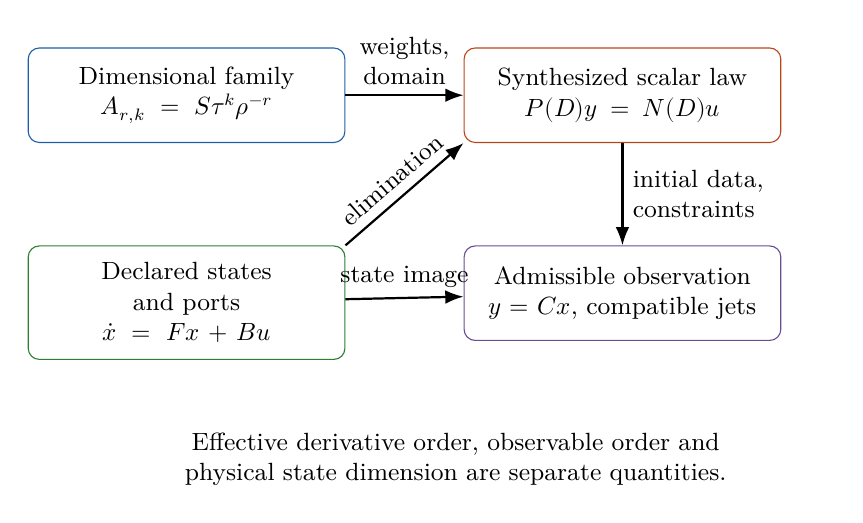
\begin{tikzpicture}[box/.style={draw,rounded corners,align=center,text width=3.6cm,minimum height=1.2cm,inner sep=6pt},>=Latex,font=\small]
\node[box,draw=elemA] (family) {Dimensional family\\$A_{r,k}=S\tau^k\rho^{-r}$};
\node[box,draw=elemB,right=1.5cm of family] (ode) {Synthesized scalar law\\$P(D)y=N(D)u$};
\node[box,draw=elemC,below=1.3cm of family] (state) {Declared states and ports\\$\dot x=Fx+Bu$};
\node[box,draw=elemD,below=1.3cm of ode] (obs) {Admissible observation\\$y=Cx$, compatible jets};
\draw[->,thick] (family)--node[above,align=center]{weights,\\domain} (ode);
\draw[->,thick] (state)--node[above,align=center]{state image} (obs);
\draw[->,thick] (state.north east)--node[sloped,above]{elimination} (ode.south west);
\draw[->,thick] (ode)--node[right,align=left]{initial data,\\constraints} (obs);
\node[align=center,below=.8cm of state.south east,anchor=north,text width=9.4cm,xshift=1.4cm] {Effective derivative order, observable order and physical state dimension\ are separate quantities.};
\end{tikzpicture}
\end{document}
